\clearpage

\begin{appendices}

\section{Final Prototype Photos}
\label{appendices:guitarimages}
\centering
\begin{figure}[h]
    \centering
    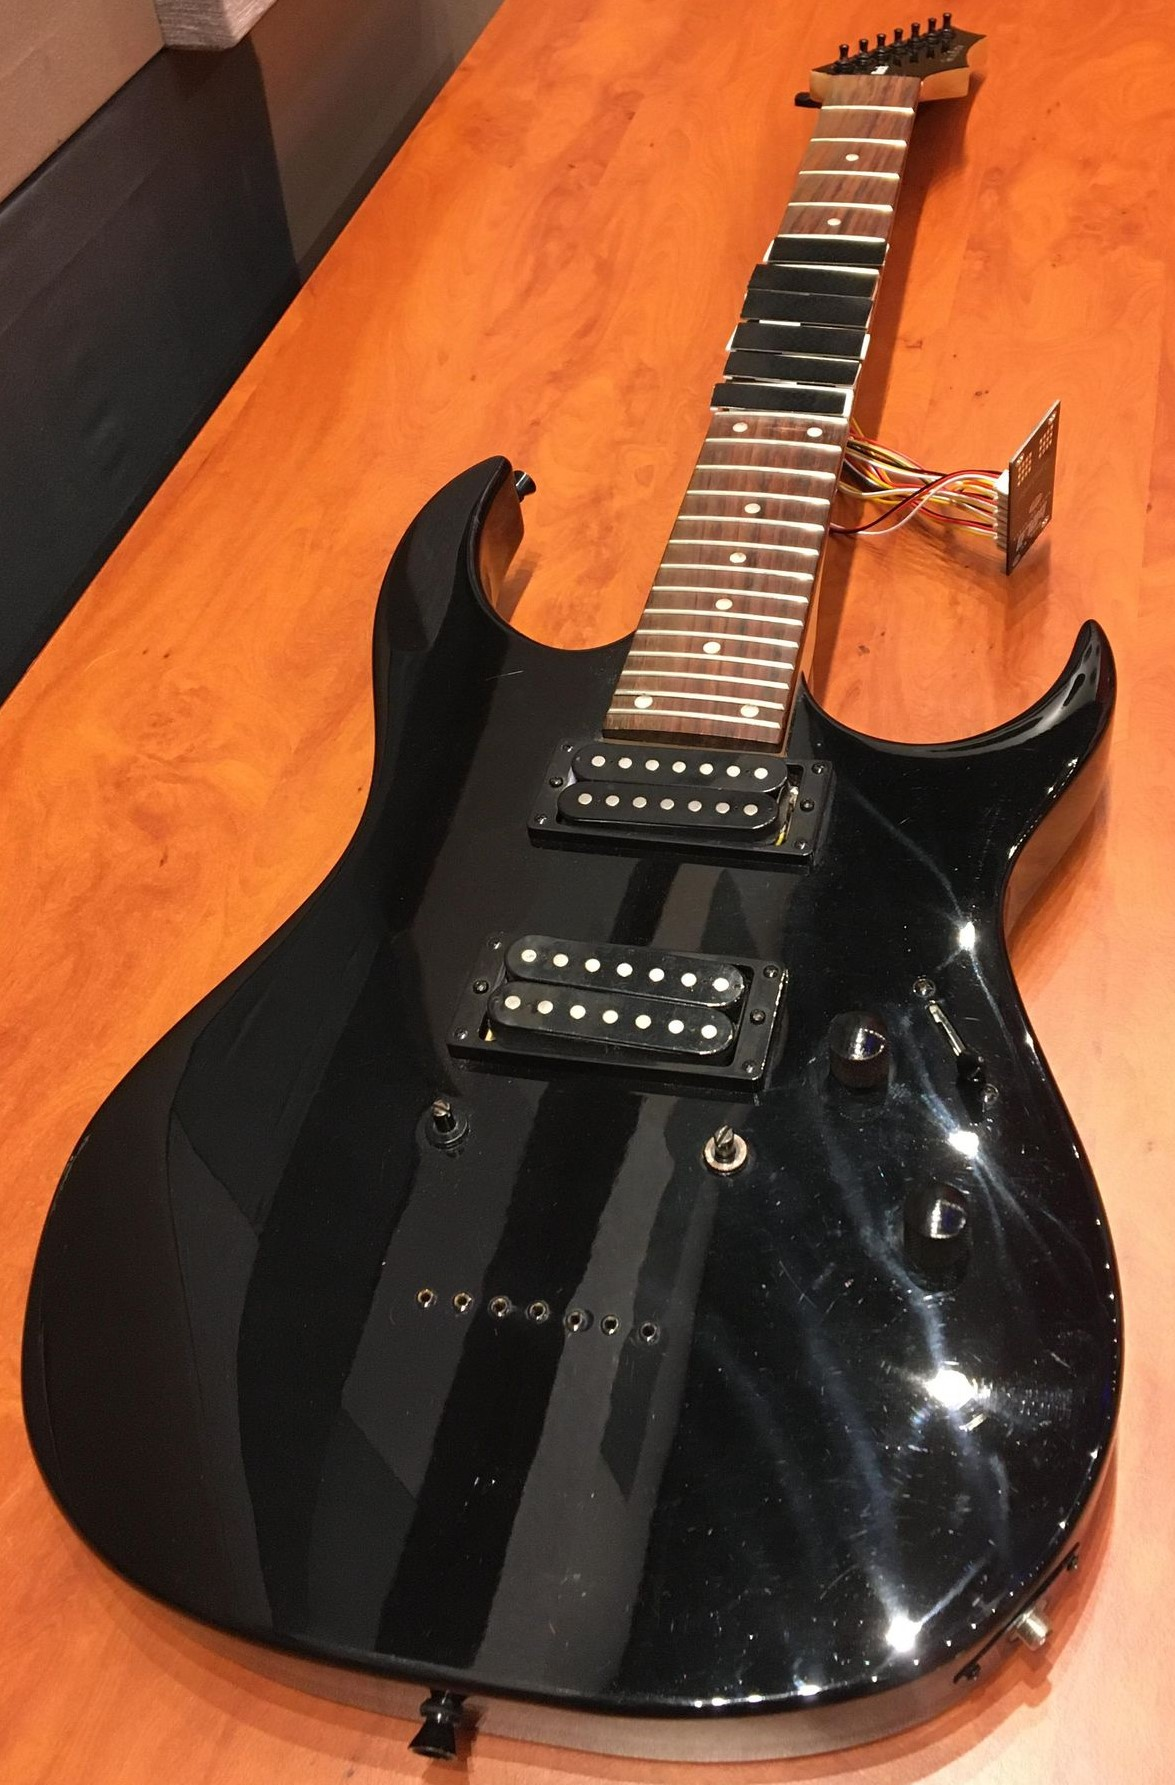
\includegraphics[scale=0.25]{Images/guitargui.jpg}
    \caption{Front of the prototype.}
    \label{fig:my_label}
\end{figure}
\begin{figure}[h]
    \centering
    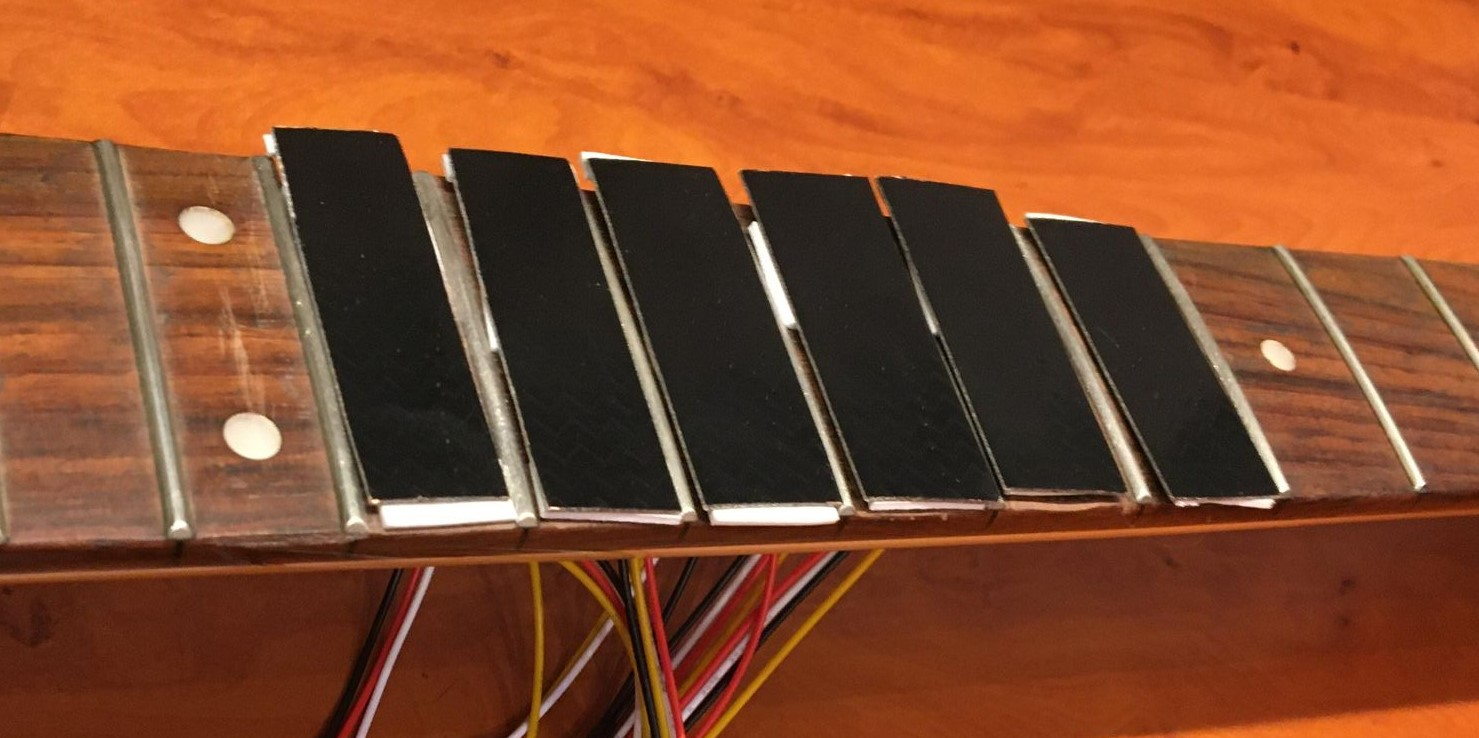
\includegraphics[scale=0.2]{Images/neck.jpg}
    \caption{Close-up of neck sensors.}
    \label{fig:my_label}
\end{figure}
\begin{figure}[h]
    \centering
    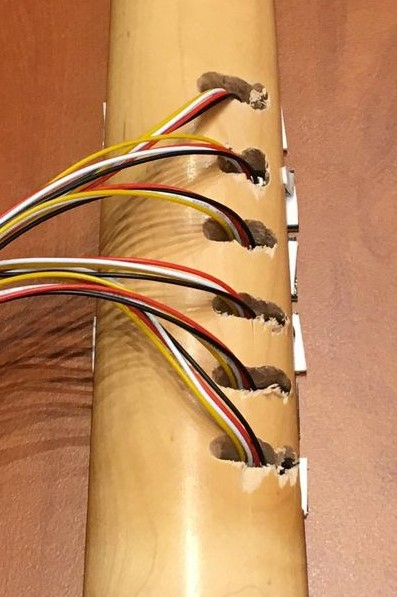
\includegraphics[scale=0.6]{Images/back.jpg}
    \caption{Back of the neck, to show I2C wiring to the sensors.}
    \label{fig:my_label}
\end{figure}

\clearpage
\section{Nielsen Usability Heuristics}
\label{appendix:heuristics}
\begin{enumerate}
    \item \textbf{Visibility of system status}: does the design keep the user informed about what is going on? 
    \item \textbf{Match between the system and the real world}: does the design follow real-world conventions and use phrases and concepts which are familiar to the user?
    \item \textbf{User control and freedom}: are users able to easily correct mistakes? This helps foster a sense of freedom and confidence in the user. 
    \item \textbf{Consistency and standards}: does the design follow platform and industry standards/conventions?
    \item \textbf{Error prevention}: it is important to let the user know when things have gone wrong, but it is even better to help prevent errors in the first place. Does the design help prevent common errors from happening?
    \item \textbf{Recognition rather than recall}: does the design minimise the user's memory load by making the interface as available as possible? Does the user have to remember different parts of the interface are hidden in deep context menus?
    \item \textbf{Flexibility and efficiency of use}: does the design offer shortcuts to expert users such that they may be able to speed up their workflow, but at the same time allowing novice users to access all the features at their own pace?
    \item \textbf{Aesthetic and minimal design}: does the interface contain information which is not needed? Interfaces should aim to minimise irrelevant information, since this reduces the relative visibility of important, relevant information.
    \item \textbf{Help users recognise, diagnose and recover from errors}: are errors expressed in plain and simple language? Does the system precisely indicate problems and suggest solutions?
    \item \textbf{Help and documentation}: does the system require additional documentation? Though it's best if the system doesn't need additional explanation, if this \textit{is} required, does the system offer this help?
\end{enumerate}









\end{appendices}